\documentclass[12pt]{article}
\usepackage{amsmath}
\usepackage{amssymb}
\usepackage{tikz}
\usepackage{geometry}
\geometry{a4paper, margin=1in}

\title{\textbf{Geometry}}\\
\author{Tutoring Centre Ferndale\\

\includegraphics[width=4em]{ApS_logo.png}}
\date{}

\begin{document}

\maketitle

\section*{Introduction}
Geometry is a branch of mathematics concerned with the properties and relations of points, lines, surfaces, and solids. It is divided into several subfields, including plane geometry, solid geometry, and coordinate geometry.

\section*{Basic Definitions}

\subsection*{Point}
A point is an exact location in space with no size, dimension, or shape. It is typically represented by a dot and labeled with a capital letter.

\subsection*{Line}
A line is a one-dimensional figure that extends infinitely in both directions. It is defined by two distinct points and is typically represented by a straight line with arrows at both ends.

\subsection*{Line Segment}
A line segment is a portion of a line that has two endpoints. It is the straight path connecting these two points.

\subsection*{Ray}
A ray starts at a point and extends infinitely in one direction. It has a fixed starting point and no endpoint.

\subsection*{Angle}
An angle is formed by two rays (called the sides of the angle) that share a common endpoint (called the vertex). The measure of an angle is typically given in degrees or radians.

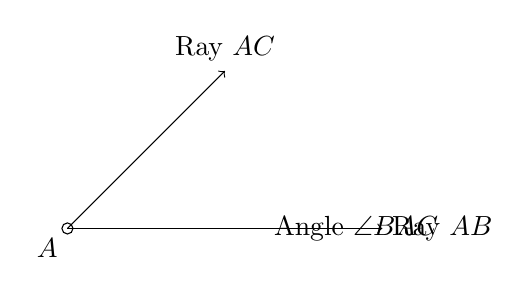
\begin{tikzpicture}
    \draw[->] (0,0) -- (4,0) node[right] {$\text{Ray } AB$};
    \draw[->] (0,0) -- (2,2) node[above] {$\text{Ray } AC$};
    \draw (0,0) circle (2pt) node[below left] {$A$};
    \draw (2.5,0) node[right] {Angle $\angle BAC$};
\end{tikzpicture}

\section*{Key Concepts}

\subsection*{Parallel Lines}
Parallel lines are lines in a plane that never intersect, no matter how far they are extended.

\subsection*{Perpendicular Lines}
Perpendicular lines intersect at a right angle (90 degrees).

\subsection*{Triangles}
A triangle is a three-sided polygon. The sum of the interior angles of a triangle is always 180 degrees. There are various types of triangles:

\begin{itemize}
    \item \textbf{Equilateral Triangle:} All three sides and angles are equal.
    \item \textbf{Isosceles Triangle:} Two sides and two angles are equal.
    \item \textbf{Scalene Triangle:} All sides and angles are different.
\end{itemize}

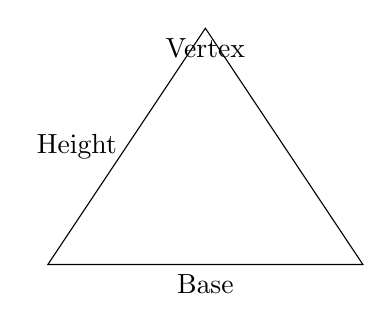
\begin{tikzpicture}
    \draw (0,0) -- (4,0) -- (2,3) -- cycle;
    \draw (2,0) node[below] {Base};
    \draw (1,1.5) node[left] {Height};
    \draw (2,2.5) node[above] {Vertex};
\end{tikzpicture}

\subsection*{Quadrilaterals}
A quadrilateral is a four-sided polygon. Some common types are:

\begin{itemize}
    \item \textbf{Square:} All sides and angles are equal.
    \item \textbf{Rectangle:} Opposite sides are equal, and all angles are right angles.
    \item \textbf{Parallelogram:} Opposite sides are parallel and equal in length.
    \item \textbf{Trapezoid:} Only one pair of opposite sides are parallel.
\end{itemize}

\begin{tikzpicture}
    \draw (0,0) -- (4,0) -- (4,3) -- (0,3) -- cycle;
    \draw (2,0) node[below] {Base};
    \draw (2,3) node[above] {Top};
    \draw (0,1.5) node[left] {Height};
\end{tikzpicture}

\subsection*{Circles}
A circle is a set of all points in a plane that are equidistant from a fixed point, called the center. Key terms include:

\begin{itemize}
    \item \textbf{Radius:} The distance from the center to any point on the circle.
    \item \textbf{Diameter:} A line segment passing through the center with endpoints on the circle (twice the radius).
    \item \textbf{Circumference:} The distance around the circle.
    \item \textbf{Arc:} A part of the circumference.
    \item \textbf{Chord:} A line segment connecting two points on the circle.
\end{itemize}

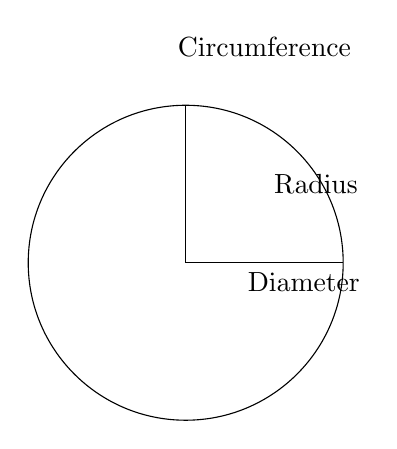
\begin{tikzpicture}
    \draw (0,0) circle (2);
    \draw (0,0) -- (2,0);
    \draw (0,0) -- (0,2);
    \draw (1,1) node[right] {Radius};
    \draw (1.5,0) node[below] {Diameter};
    \draw (1,2.5) node[above] {Circumference};
\end{tikzpicture}

\section*{Examples and Applications}

\subsection*{Example 1: Finding the Area of a Triangle}
To find the area of a triangle, use the formula:
\[
\text{Area} = \frac{1}{2} \times \text{base} \times \text{height}
\]
Given a triangle with a base of 5 cm and a height of 4 cm:
\[
\text{Area} = \frac{1}{2} \times 5 \, \text{cm} \times 4 \, \text{cm} = 10 \, \text{cm}^2
\]

\subsection*{Example 2: Finding the Circumference of a Circle}
To find the circumference of a circle, use the formula:
\[
\text{Circumference} = 2 \pi \times \text{radius}
\]
Given a circle with a radius of 7 cm:
\[
\text{Circumference} = 2 \pi \times 7 \, \text{cm} \approx 43.98 \, \text{cm}
\]

\section*{Conclusion}
Geometry is a fundamental branch of mathematics that deals with shapes, sizes, and the properties of space. Understanding basic geometric concepts provides a foundation for more advanced topics and practical applications in various fields.

\end{document}
